\hspace{-1cm}
	\centering
	\begin{tabular}{p{4cm}p{10cm}}
		\hline
		Title & tourism app \\
		\hline
		Date & 16th April 2019 \\
		\hline
		Scene & 2 of 4 \\
		\hline
		Description & The search page of the application \\
		\hline
		Links From Scenes & Scene 1, Scene 3 \\
		\hline
		Links To Scenes & Scene 3 \\
		\hline
		\multicolumn{2}{c}{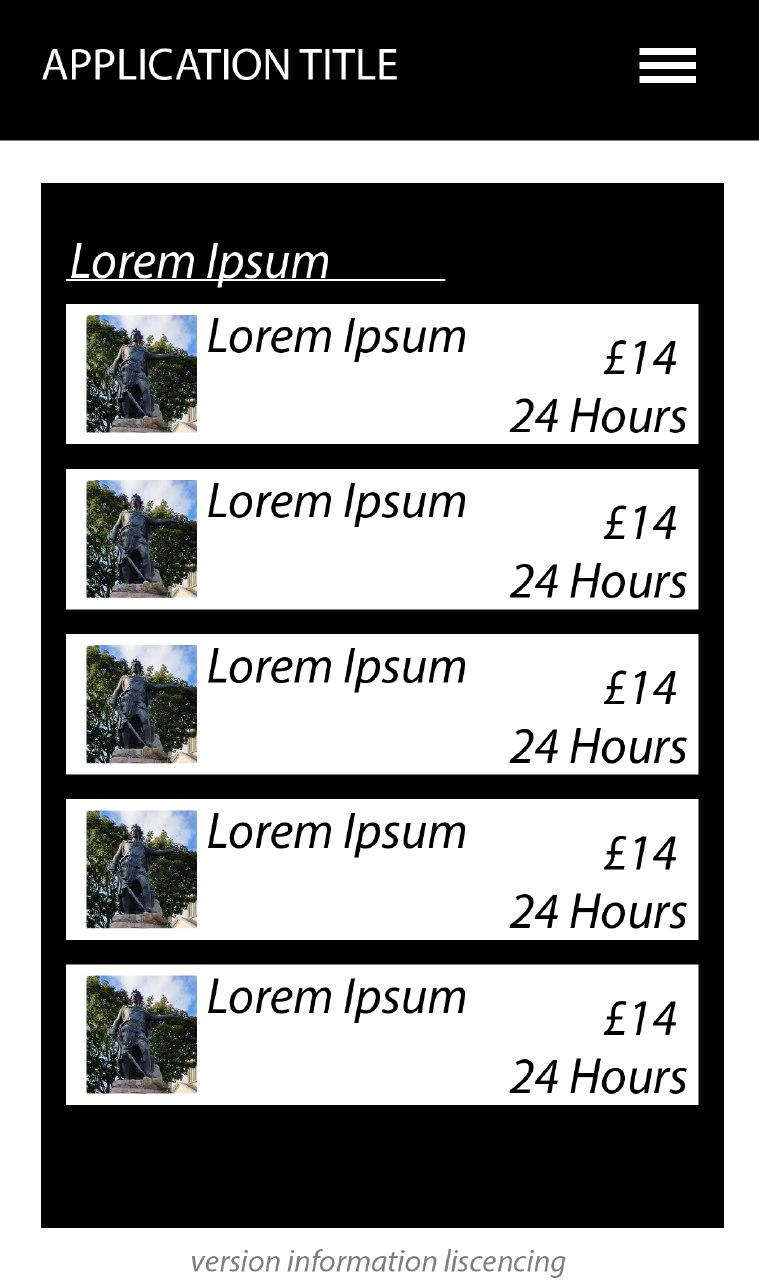
\includegraphics[width=0.5\linewidth]{images/screen1.jpg}} \\
		\hline
		Background & Standard phone background \\
		\hline
		Colour Scehemes Used & Default to black and white but would import from the system theme so users feel immersed \\
		\hline
		Text Attributes & Again, follows system theme (usually a sans-serif font). \\
		\hline
		Audio Files & N/A \\
		\hline
		Video Files & N/A \\
		\hline
		Stills Files & N/A \\
		\hline
		Animations / Movie Clips & N/A \\
		\hline
		\multicolumn{2}{c}{Interface Components (buttons, widgets)} \\
		\hline
		\multicolumn{2}{p{14cm}}{ This page shows a list of "card"-esque locations that match the search term provided by the user on the main page. Above them is the search box that the user can see their current search and make an edit to it.  } \\
		\hline
	\end{tabular}
